\documentclass{article}
\usepackage[italian]{babel}
\usepackage[a4paper, left=3.5cm, right=3.5cm, top=3cm, bottom=4cm]{geometry}
\usepackage{graphicx} % Required for inserting images
\usepackage{tcolorbox}
\usepackage{booktabs} % Per una tabella più elegante
\usepackage[hidelinks]{hyperref}
\usepackage{ffcode}
\usepackage{todonotes}
\usepackage[dvipsnames]{xcolor}

\font\myfont=cmr10 at 28pt
\setlength{\parindent}{0pt}

\hypersetup{
    colorlinks=true,
    linkcolor=NavyBlue,
    filecolor=Blue,      
    urlcolor=NavyBlue,
    citecolor=NavyBlue,
    pdftitle={WiFind: Localizzazione indoor tramite WiFi fingerprinting},
    pdfpagemode=FullScreen,
    }
\bibliographystyle{IEEEtran}

\title{{\myfont WiFind}}
\author{
    Gabriele Aprile\\
    \texttt{0001186570}
    \and
    Matteo Cardellini\\
    \texttt{0001186864}
    \and
    Andreea Scrob\\
    \texttt{0001186874}
}
\date{A.A. 2024/2025 -- March 2025}

\begin{document}

\maketitle

\begingroup
\hypersetup{hidelinks} 
\tableofcontents
\endgroup

\newpage

%%%%%%%%%%%%%%%%%%%%%%%%
\section{Introduzione}
La localizzazione degli utenti all'interno di ambienti è un problema di grande interesse in diversi ambiti, come la sicurezza, la domotica e la navigazione indoor. Una delle tecniche più usate per determinare la posizione di un utente è il \textbf{WiFi fingerprinting}\footnote{tecnica di localizzazione basata sulla raccolta e analisi delle ''impronte digitali'' dei segnali WiFi in una determinata area. Ogni posizione ha una \textit{firma} unica data dalla combinazione dei segnali ricevuti dai vari access point, che viene utilizzata per stimare la posizione dell'utente.}, che sfrutta la potenza del segnale ricevuto (RSSI\footnote{\textit{Received Signal Strength Indicator} indica la potenza del segnale ricevuto da un dispositivo, misurata in dBm (decibel rispetto a 1 mW).}) da più punti di accesso per stimare la posizione tramite modelli di machine learning.

\subsection{Descrizione del problema}
Il problema in analisi consiste nel determinare con la massima precisione possibile la posizione di un utente in un dato ambiente indoor utilizzando solo i dati di rete, evitando l'uso di hardware aggiuntivo come GPS o sensori esterni. \\

Nel nostro caso, il problema è \textit{determinare in quale stanza del Dipartimento di Informatica si trovi un dato utente}, basandoci sulle informazioni degli access point della rete universitaria AlmaWiFi.

\subsection{Soluzioni proposte}
Per affrontare il problema, si propone di:
\begin{itemize}
    \item scegliere una struttura ben definita e raccogliere i dati al suo interno, in modo da poter \textbf{creare un dataset};
    \item \textbf{selezionare un modello di machine learning} semplice ed efficace, come \textit{K-Nearest Neighbors (KNN)} o \textit{Random Forest}, per la classificazione della posizione;
    \item \textbf{valutare le metriche} e \textbf{ottimizzare il modello} in modo da ottenere risultati soddisfacenti.
\end{itemize}

\section{Metodi proposti}
\subsection{Dataset}
\subsubsection{Raccolta e preprocessing}
\begin{figure}[ht!]
    \centering
    {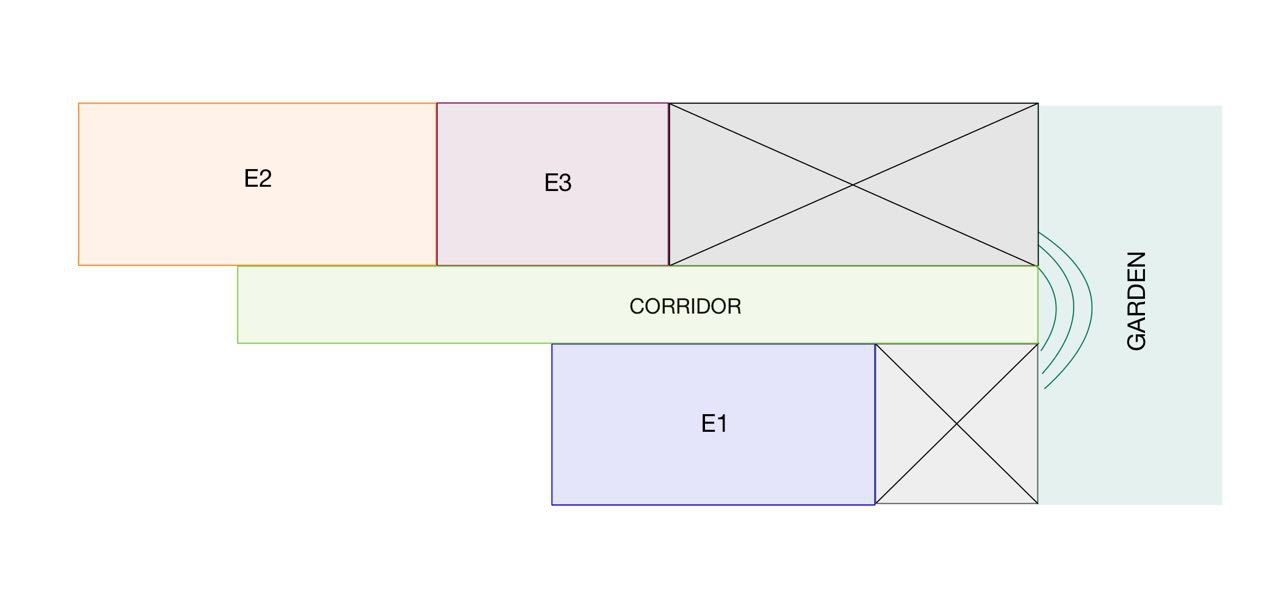
\includegraphics[scale=0.28]{img/piantinaErcolani.JPG}}
    \caption{Mappa dell’edificio Ercolani con le stanze usate per la raccolta dati}
    \label{Pianta}
\end{figure}
Si è deciso di creare un \textbf{dataset ad-hoc} per il progetto, raccogliendo i dati relativi ai vari \textit{access point} dell'edificio Ercolani (la cui cartina è visibile in \autoref{Pianta}), attraverso una serie di script Python.
Per valutare l'impatto degli ostacoli sulle onde radio, un fattore che potrebbe causare interferenze, la rilevazione è stata effettuata due volte per ogni stanza: una con la stanza vuota (\textit{Empty}) e una con la stanza affollata (\textit{Crowded}). \\
Al termine della raccolta, i dati sono stati filtrati conservando esclusivamente quelli relativi alla rete \textbf{AlmaWIFI}, come mostrato in \autoref{tab:wifi_data}.

\begin{table}[ht!]
    \centering
    \small
    \begin{tabular}{llc c c cc}
        \toprule
        Aula & Situazione & AP1 & AP2 & \dots & AP41 & AP42 \\
        \midrule
        E1 & Empty & -76.0 &  & \dots & -89.0 & \\

        E2 & Empty & -45.0 & -66.0  & \dots &  & \\
        E3 & Empty & -64.0 & -79.0 & \dots &  &  \\     
        Corridor & Empty & -48.0 & -66.0  & \dots &  & \\
        Garden & Empty &  &   & \dots &  & -91.0 \\
         \vdots & \vdots & \vdots & \vdots & \vdots & \vdots & \vdots \\
        E1 & Crowded & -84.0 &  & \dots & -91.0 &  \\
        E2 & Crowded & -47.0 & -64.0  & \dots &  & \\   
        E3 & Crowded & -66.0 & -78.0 & \dots &  &  \\
        Corridor & Crowded &  & -93.0  & \dots &  & \\
        Garden & Crowded & -78.0 &   & \dots &  & \\

        \bottomrule
    \end{tabular}
    \caption{Estratto del dataset \textit{wifi\_fingerprinting\_dataset\_raw.csv} }
    \label{tab:wifi_data}
\end{table}

\subsubsection{Analisi Esplorativa dei dati}
Grazie al supporto di grafici, sono state condotte analisi preliminari sui dati raccolti.\\
In particolare, è stato realizzato un \textbf{istogramma} per esaminare il numero totale di segnali rilevati da ciascun access point (AP) (vedi \autoref{FreqAP}).
È stata inoltre generata una \textbf{heatmap} (\autoref{heatmap}) della potenza del segnale Wi-Fi, che evidenzia l'intensità media rilevata per ogni AP all'interno di diverse aree (E1, E2, E3, Corridoio, Giardino), nelle due differenti condizioni ambientali (Empty, Crowded). I colori della mappa riflettono visivamente la forza del segnale ricevuto.\\
Questi grafici hanno permesso una comprensione più chiara della struttura del dataset, evidenziando come alcuni access point risultassero poco significativi a causa del numero esiguo di rilevazioni associate, suggerendo la necessità di effettuare ulteriori operazioni di pulizia e selezione dei dati.

\begin{figure}[ht!]
    \centering
    {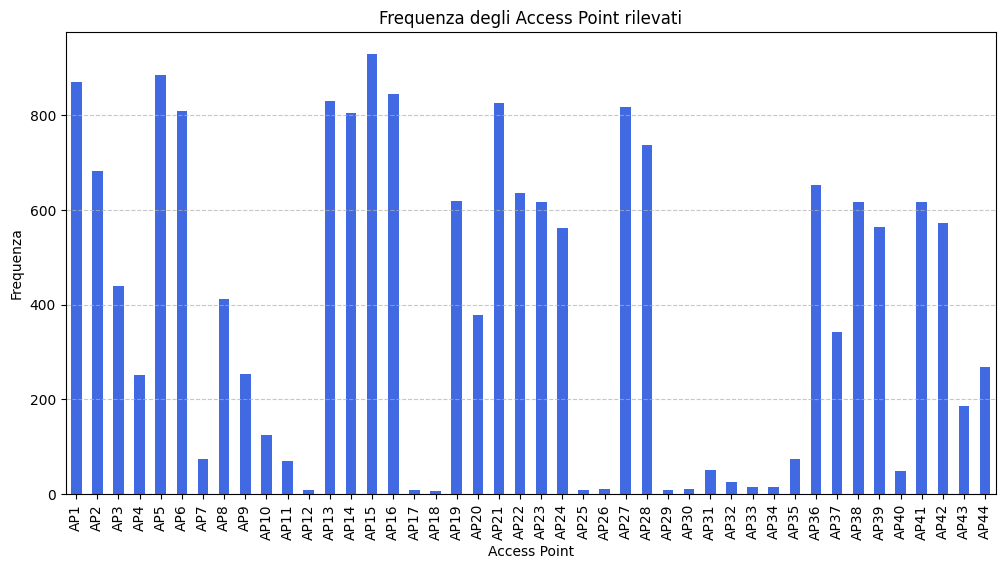
\includegraphics[scale=0.50]{img/output.png}}
    \caption{Istogramma del numero totale di rilevazioni per ciascun Access Point (AP)}
    \label{FreqAP}
\end{figure}

\begin{figure}[ht!]
    \centering
    {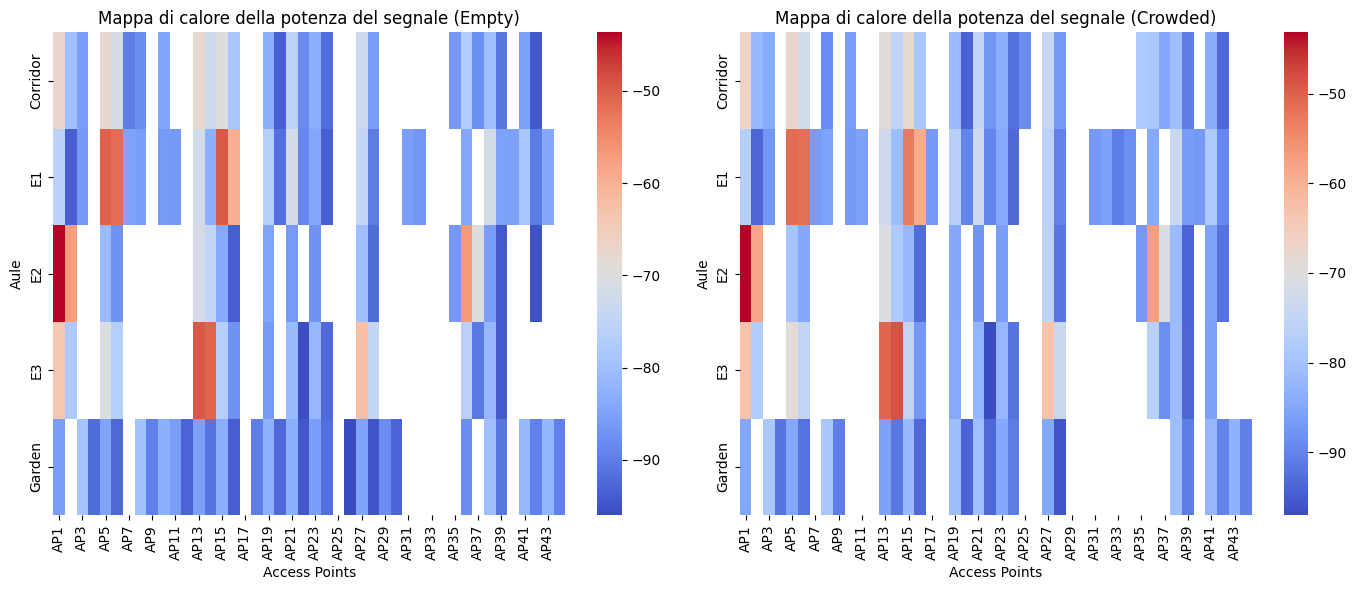
\includegraphics[scale=0.38]{img/ColorMap.png}}
    \caption{Heatmap della potenza media del segnale Wi-Fi nelle condizioni \textit{Empty} e \textit{Crowded}}
    \label{heatmap}
\end{figure}

\subsubsection{Manipolazioni del dataset}
Come detto in precedenza, si è notato come alcuni access point venissero rilevati meno frequentemente rispetto ad altri (\autoref{FreqAP}). Per questo motivo, si è scelto di \textbf{ridurre la presenza di AP} poco rappresentativi nel dataset. A tale scopo, è stato utilizzato uno script Python che ha rimosso tutti gli AP con meno di 400 rilevazioni, mantenendo inalterati gli altri. Il dataset ottenuto viene indicato con il nome \textbf{cut400}.\\
Questa operazione ha avuto anche l’effetto positivo di rendere il dataset più “verticale", ovvero con un numero più contenuto di feature (access point) rispetto al numero totale di istanze. In questo modo, si è ridotto il rischio di sovradimensionamento dello spazio delle feature, che potrebbe altrimenti compromettere l'efficacia di modelli come KNN. \\

Sono stati generati ulteriori dataset, tra cui uno con \textit{valori normalizzati} e uno con \textit{valori binarizzati}.\\
Nel primo caso, denominato \textbf{normalized}, ogni valore di potenza RSSI è stato scalato in un intervallo compreso tra 0 e 1, con una precisione di 16 cifre decimali. Per la normalizzazione è stato adottato il metodo Min-Max, secondo la formula:
\[X_{norm}= \frac{X-X_{min}}{X_{max}-X_{min}}\] \\
Nel dataset binarizzato, chiamato \textbf{binarized}, l'obiettivo è invece quello di rappresentare la semplice presenza o assenza del segnale, piuttosto che la sua intensità. A tal fine, i valori RSSI sono stati convertiti in binari: in presenza di segnale è stato assegnato il valore \textbf{1}, in assenza il valore \textbf{0}. Il risultato di questa trasformazione è mostrato in \autoref{tab:wifi_data_bin}. \\

\begin{table}[ht!]
    \centering
    \small
    \begin{tabular}{llc c c cc}
        \toprule
        Aula & Situazione & AP1 & AP2 & \dots & AP41 & AP42 \\
        \midrule
        E1 & Empty & 1 & 0 & \dots & 1 & 0 \\
        E2 & Empty & 1 & 1  & \dots & 0 & 0\\
        E3 & Empty & 1 & 1 & \dots & 0 & 0 \\     
        Corridor & Empty & 1 & 1  & \dots & 0 &0 \\
        Garden & Empty & 0 & 0  & \dots &  0& 1\\
         \vdots & \vdots & \vdots & \vdots & \vdots & \vdots & \vdots \\
        E1 & Crowded & 1 & 0 & \dots & 1 & 0 \\
        E2 & Crowded & 1 & 1  & \dots & 0 & 0\\   
        E3 & Crowded & 1 & 1 & \dots & 0 & 0 \\
        Corridor & Crowded & 0 & 1  & \dots & 0 & 0\\
        Garden & Crowded & 1 & 0  & \dots & 0 & 0\\
        \bottomrule
    \end{tabular}
    \caption{Estratto del file \textit{wifi\_fingerprinting\_dataset\_binarized.csv}}
    \label{tab:wifi_data_bin}
\end{table}

È importante sottolineare che, per rendere \textit{cut400} compatibile con l'addestramento dei modelli, i campi privi di rilevazioni sono stati sostituiti con il valore \textbf{-200}, un valore fittizio che rappresenta ``un access point troppo distante per essere rilevato''. \\
Questo ragionamento non viene ovviamente applicato per \textit{binarized} e \textit{normalized}, che per sua natura hanno tutti i campi contenenti un valore.\\

Ulteriori motivazioni e considerazioni riguardanti l'utilizzo di questi dataset alternativi verranno approfondite successivamente.

\begin{figure}[ht!]
    \centering
    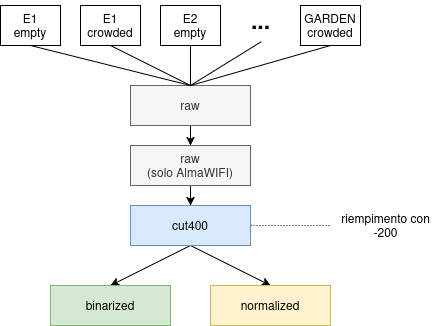
\includegraphics[width=0.5\linewidth]{img/datasetHistory.png}
    \caption{Schema dell’evoluzione del dataset: da raw a cut400, normalized e binarized}
    \label{fig:datasetHistory}
\end{figure}



\subsection{Modelli}
Sin dall'inizio, abbiamo adottato un approccio metodologico basato sulle conoscenze acquisite nel nostro percorso accademico, al fine di strutturare e avviare il lavoro in modo rigoroso. \\

Dato il problema di \textbf{classificazione} da risolvere, come primo passo, abbiamo scelto di procedere ad una prima implementazione di \textbf{K-Nearest Neighbors} (\textbf{KNN}), un modello di machine learning noto per la sua semplicità ed efficacia, frequentemente incontrato e studiato nel corso della nostra formazione.
Il \textbf{KNN} è un algoritmo supervisionato basato sul principio della vicinanza: classifica un nuovo dato assegnandogli l'etichetta predominante tra i suoi \textbf{k} vicini più prossimi, misurati tramite diverse metriche. La scelta di questo modello iniziale ci ha permesso di stabilire un punto di riferimento per valutare le prestazioni e l'affidabilità dei successivi approcci sperimentati.\\
L'analisi è stata approfondita tramite l’uso di algoritmi più raffinati, come ad esempio il Random Forest. \\

Dopo diversi tentativi e ricerche, è stata trovata una pubblicazione \cite{Shang2022} che affronta in modo specifico il problema della localizzazione indoor tramite WiFi fingerprinting.\\
Nel paper viene condotta un'analisi comparativa tra diversi algoritmi di Machine Learning, evidenziandone i punti di forza e le limitazioni in relazione a questo specifico contesto applicativo.\\
Vengono citati:
\begin{itemize}
    \item \textbf{K-Nearest Neighbour (KNN)}: particolarmente adatto a dataset di dimensioni moderate, e relativamente semplice da implementare e regolare. Tuttavia non è consigliato per dataset con un elevato numero di feature, poiché la sua efficienza può risentirne.
    \item \textbf{Support Vector Machine (SVM)}: efficace su dataset ad alta dimensionalità, grazie alla sua capacità di trovare iperpiani di separazione ottimali tra le classi. Ciononostante, può risultare meno performante in presenza di numerosi outlier o quando le classi sono fortemente sovrapposte nello spazio delle feature, rendendo difficile la separazione dei cluster.
    \item \textbf{Random Forest}: particolarmente indicato per dataset di grandi dimensioni, grazie alla sua robustezza e capacità di generalizzazione. Essendo un metodo basato su un insieme di alberi decisionali, riesce a ridurre il rischio di overfitting e a garantire una maggiore stabilità nelle predizioni.
\end{itemize}

Considerando i nostri dataset di dimensioni non eccessive e di dimensionalità mai superiori a 44 (massimo numero di AP individuati), si è deciso di procedere utilizzando il modello \textit{KNN}, puntando ad un miglioramento tramite \textit{tuning} di parametri.\\
Qualora il KNN non si fosse rivelato sufficientemente performante, avremmo proceduto con un'analisi più approfondita di altri modelli di classificazione, al fine di individuare soluzioni più efficaci per il problema affrontato.

%%%%%
\subsection{K-Nearest Neighbors}
\subsubsection{Divisione dataset}
Al fine di verificare la robustezza del modello nelle varie possibili situazioni di affollamento delle stanze, il dataset è stato manipolato per ottenere tre dataframe diversi, corrispondenti alle situazioni “\textbf{Empty}" (aula vuota), “\textbf{Crowded}" (aula affollata) e “\textbf{Hybrid}" (situazione mista, ovvero l'unione dei due dataframe precedenti).\\
Per gestire correttamente la fase di addestramento e valutazione, si è definita la funzione \textit{split\_data}, che divide ogni sottoinsieme in un \textbf{training set} (70\% dei dati) e un \textbf{test set} (30\% dei dati). Questa suddivisione avviene in modo \textbf{stratificato}, ovvero mantenendo la distribuzione originale delle classi.\\
Il \textit{validation set} non è stato separato esplicitamente in questa fase, ma il suo utilizzo è garantito tramite una tecnica descritta nel paragrafo seguente.


\subsubsection{Ottimizzazione del Modello}
Durante lo studio per migliorare le prestazioni del modello KNN, ci siamo imbattuti in diversi approcci affrontati dalla letteratura del caso, come ad esempio quello presentato in \cite{electro}: il metodo Weighted k-Nearest Neighbors (WKNN) permette di utilizzare metriche di distanza più sofisticate e migliorare la selezione dei vicini. \\
Tuttavia, abbiamo scelto un approccio più tradizionale e consolidato: \textbf{Grid Search}, che consente una ricerca sistematica degli iperparametri ottimali.\\

\textbf{Grid Search: ricerca degli iperparametri ottimali}\\\\
La \textit{Grid Search} è una tecnica utilizzata per individuare la combinazione ottimale di \textbf{iperparametri}\footnote{Parametri che non vengono appresi dal modello, ma devono essere definiti a priori.} di un algoritmo di machine learning.  
Nel nostro caso, è stata impiegata per ottimizzare le prestazioni del modello KNN, esplorando sistematicamente diverse configurazioni degli iperparametri.

Il processo si articola in tre fasi principali:
\begin{enumerate}
    \item definizione di una griglia di valori possibili per ciascun iperparametro del modello;
    \item addestramento del modello su tutte le combinazioni possibili della griglia;
    \item valutazione delle prestazioni di ogni combinazione tramite una metrica predefinita (es. accuratezza), e selezione della migliore configurazione.
\end{enumerate}

Nel nostro progetto, la griglia dei valori esplorata è riportata nella \autoref{tab:param_grid}.

\begin{table}[ht!]
\centering
\begin{tabular}{ll}
\toprule
\textbf{Parametro} & \textbf{Valori esplorati} \\
\midrule
\texttt{n\_neighbors} & 3--19 \\
\texttt{weights} & \texttt{['uniform', 'distance']} \\
\texttt{algorithm} & \texttt{['ball\_tree', 'brute']} \\
\texttt{metric} & \texttt{['euclidean', 'manhattan']} \\
\bottomrule
\end{tabular}
\caption{Griglia dei valori esplorati tramite Grid Search}
\label{tab:param_grid}
\end{table}

Di seguito una panoramica dei parametri ottimizzati:

\begin{itemize}
    \item \textbf{n\_neighbors} -- rappresenta il valore di $K$ in KNN, ovvero il numero di vicini da considerare per effettuare la classificazione.
    \begin{itemize}
        \item Un valore di $K$ troppo basso può portare a \textit{overfitting}, mentre valori troppo alti rischiano di causare \textit{underfitting}.
        \item \underline{Valutazione}: Il range 3--19 è stato ritenuto un buon compromesso per bilanciare queste problematiche.
    \end{itemize}
    
    \item \textbf{weights} -- specifica l'importanza assegnata ai vicini nel processo decisionale.
    \begin{itemize}
        \item \textit{uniform}: tutti i vicini contribuiscono in egual misura.
        \item \textit{distance}: i vicini più prossimi hanno un peso maggiore.
        \item \underline{Valutazione}: Considerando la natura dei dati, l'opzione \textit{uniform} potrebbe essere sufficiente, ma si è lasciata comunque la scelta aperta.
    \end{itemize}
    
    \item \textbf{algorithm} -- metodo utilizzato per calcolare i vicini più prossimi.
    \begin{itemize}
        \item \textit{ball\_tree}: adatto a dataset di dimensioni medio-grandi e con molte feature sparse.
        \item \textit{brute}: approccio esaustivo che calcola la distanza tra tutte le coppie di punti; adatto a dataset piccoli.
        \item \textit{kd\_tree}: efficiente con dataset bilanciati e a bassa dimensionalità.
        \item \underline{Valutazione}: Considerate le dimensioni contenute del dataset, \textit{ball\_tree} e \textit{brute} sono risultati i più adatti.
    \end{itemize}
    
    \item \textbf{metric} -- criterio di distanza utilizzato per calcolare la somiglianza tra i punti.
    \begin{itemize}
        \item \textit{euclidean}: la distanza euclidea classica tra punti nello spazio.
        \item \textit{manhattan}: somma delle distanze assolute per ogni dimensione; più robusta in spazi ad alta dimensionalità.
        \item \textit{minkowski}: generalizzazione delle due precedenti.
        \item \underline{Valutazione}: Dato il numero limitato di feature, si è scelto di testare soltanto le metriche \textit{euclidean} e \textit{manhattan}.
    \end{itemize}
\end{itemize}

Altri iperparametri disponibili per il modello KNN, ma ritenuti meno influenti nel nostro contesto, sono stati lasciati ai valori di default:
\begin{itemize}
    \item \textbf{p} -- esponente utilizzato nella metrica Minkowski.
    \item \textbf{leaf\_size} -- numero massimo di punti che possono essere contenuti in una foglia degli alberi (\textit{ball\_tree} e \textit{kd\_tree}).
\end{itemize}

\textbf{Cross Validation: validazione robusta delle scelte sui parametri
}\\\\
La Grid Search è implementata nel codice tramite la funzione \textit{GridSearchCV} del pacchetto Scikit-Learn. Questa funzione consente di individuare la combinazione ottimale di iperparametri attraverso una valutazione basata su \textit{validation test}. 
In particolare, sfrutta la tecnica della \textbf{Cross Validation}, suddividendo il dataset di addestramento in K sottoinsiemi (\textit{fold}), eseguendo il training del modello K volte:
\begin{itemize}
    \item Ad ogni iterazione, K-1 folds vengono usati per l'addestramento e il fold rimanente è considerato come validation set.
    \item Alla fine, si calcola la media delle prestazioni, ottenendo una valutazione più stabile e affidabile.
\end{itemize}

Abbiamo scelto di utilizzare la \textit{Stratified K-Fold Cross Validation}, in quanto garantisce che ogni fold mantenga le stesse proporzioni delle classi presenti nel dataset originale. Questo è particolarmente importante quando le classi sono sbilanciate, poiché assicura che la distribuzione dei dati sia coerente in tutte le iterazioni.\\

L'integrazione di Grid Search con Cross Validation ha permesso di \textbf{ottimizzare il modello in modo rigoroso}, migliorandone l'affidabilità e la capacità di generalizzare su nuovi dati.


\subsubsection{Metriche}
Dopo aver trovato i migliori parametri, il modello viene testato e valutato su diverse metriche:
\begin{itemize}
    \item \textbf{Accuracy}: misura la quantità di elementi correttamente classificati (veri positivi e veri negativi) sul totale delle previsioni.
    \item \textbf{Precision}: misura la quantità di elementi correttamente classificati come positivi (veri positivi) sul totale di tutti i positivi (veri positivi e falsi positivi).
    \item \textbf{Recall}: misura quanto bene il modello riesce a trovare tutti i veri positivi (sull'insieme di veri positivi e falsi negativi).
    \item \textbf{F1-score}: è la media armonica tra Precision e Recall.
\end{itemize}


%%%%%%%%%%%%%%%%%%%%%%
\section{Risultati e Commenti}
Dopo aver testato il sistema sui diversi dataset, abbiamo ritenuto più significativo utilizzare il \textbf{dataset \textit{binarized}}, in cui i segnali sono rappresentati in termini di presenza o assenza (1/0), anziché attraverso i valori esatti di intensità (RSSI).\\

Questa scelta è stata motivata dal sospetto di \textit{overfitting} riscontrato nei modelli addestrati con i dataset alternativi contenenti valori RSSI. La nostra ipotesi è che fornire al sistema valori di intensità troppo precisi, a fronte di un dataset relativamente ridotto, induca il modello a cogliere pattern eccessivamente specifici, compromettendone la capacità di generalizzazione su dati nuovi.\\

La generalizzazione introdotta dal formato binario ha inoltre reso i test qualitativamente più significativi, evidenziando con maggiore chiarezza la complessità del problema e le differenze tra le classi.

\subsection{Training}
Utilizzando GridSearchCV, abbiamo trovato gli iperparametri ideali per ognuno dei tre scenari Empty, Crowded e Hybrid, ottenendo i risultati riportati nella \autoref{tab:best_params}. \\
\begin{table}[ht!]
    \centering
    \begin{tabular}{ c c c c c c}
        \hline
        \textbf{Scenario} & \textbf{Algorithm} & \textbf{Metric} & \textbf{Neighbors} & \textbf{Weights} & \textbf{Best Accuracy} \\
        \hline
        Empty   & brute         & manhattan & 6  & distance & 0.9793  \\
        Crowded & ball\_tree    & manhattan & 15 & distance & 0.9340    \\
        Hybrid  & brute         & euclidean & 16 & uniform  & 0.9302     \\
        \hline
    \end{tabular}
    \caption{Configurazioni ottimali del modello KNN per i tre scenari, con relative accuratezze}
    \label{tab:best_params}
\end{table}

È interessante notare come per ben due scenari l'algoritmo usato sia di tipo \textit{brute force}, a dimostrazione del fatto che le dimensioni relativamente contenute del dataset consentono il calcolo delle distanze tra tutte le coppie di punti. Per quanto riguarda le metriche, in due casi su tre è stata scelta la \textit{manhattan}, attestando una tendenza del dataset a presentarsi come ``largo", ovvero con un numero considerevole di features.\\
Si è proceduto ad addestrare il modello usando gli iperparametri trovati.

\subsection{Testing}
Per testare in modo più rigoroso il modello, si è deciso di valutarlo su tutte le possibili combinazioni ambientali, come riportato in \autoref{tab:model_metrics}.
Ad ogni combinazione sono stati associati i relativi valori delle metriche precedentemente discussi.

\begin{table}[ht!]
    \centering

    \begin{tabular}{c c c c c c }
        \hline
         \textbf{Train Model} & \textbf{Test Model} & Accuracy & Precision & Recall & F1-score \\
        \hline
        Empty   & Empty   & 0.932 & 0.935 & 0.932 & 0.931 \\
        Empty   & Crowded & 0.813 & 0.808 & 0.813 & 0.797 \\
        Empty   & Hybrid  & 0.912 & 0.912 & 0.912 & 0.909 \\
        Crowded & Empty   & 0.904 & 0.913 & 0.904 & 0.904 \\
        Crowded & Crowded & 0.887 & 0.884 & 0.887 & 0.884 \\
        Crowded & Hybrid  & 0.919 & 0.922 & 0.919 & 0.919 \\
        Hybrid  & Empty   & 0.959 & 0.962 & 0.959 & 0.959 \\
        Hybrid  & Crowded & 0.907 & 0.905 & 0.907 & 0.905 \\
        Hybrid  & Hybrid  & 0.929 & 0.933 & 0.929 & 0.929 \\
        \hline
    \end{tabular}
    \caption{Valutazione del modello KNN: metriche per tutte le combinazioni di training e test}
    \label{tab:model_metrics}
\end{table}

\begin{figure}[ht!]
    \centering
    {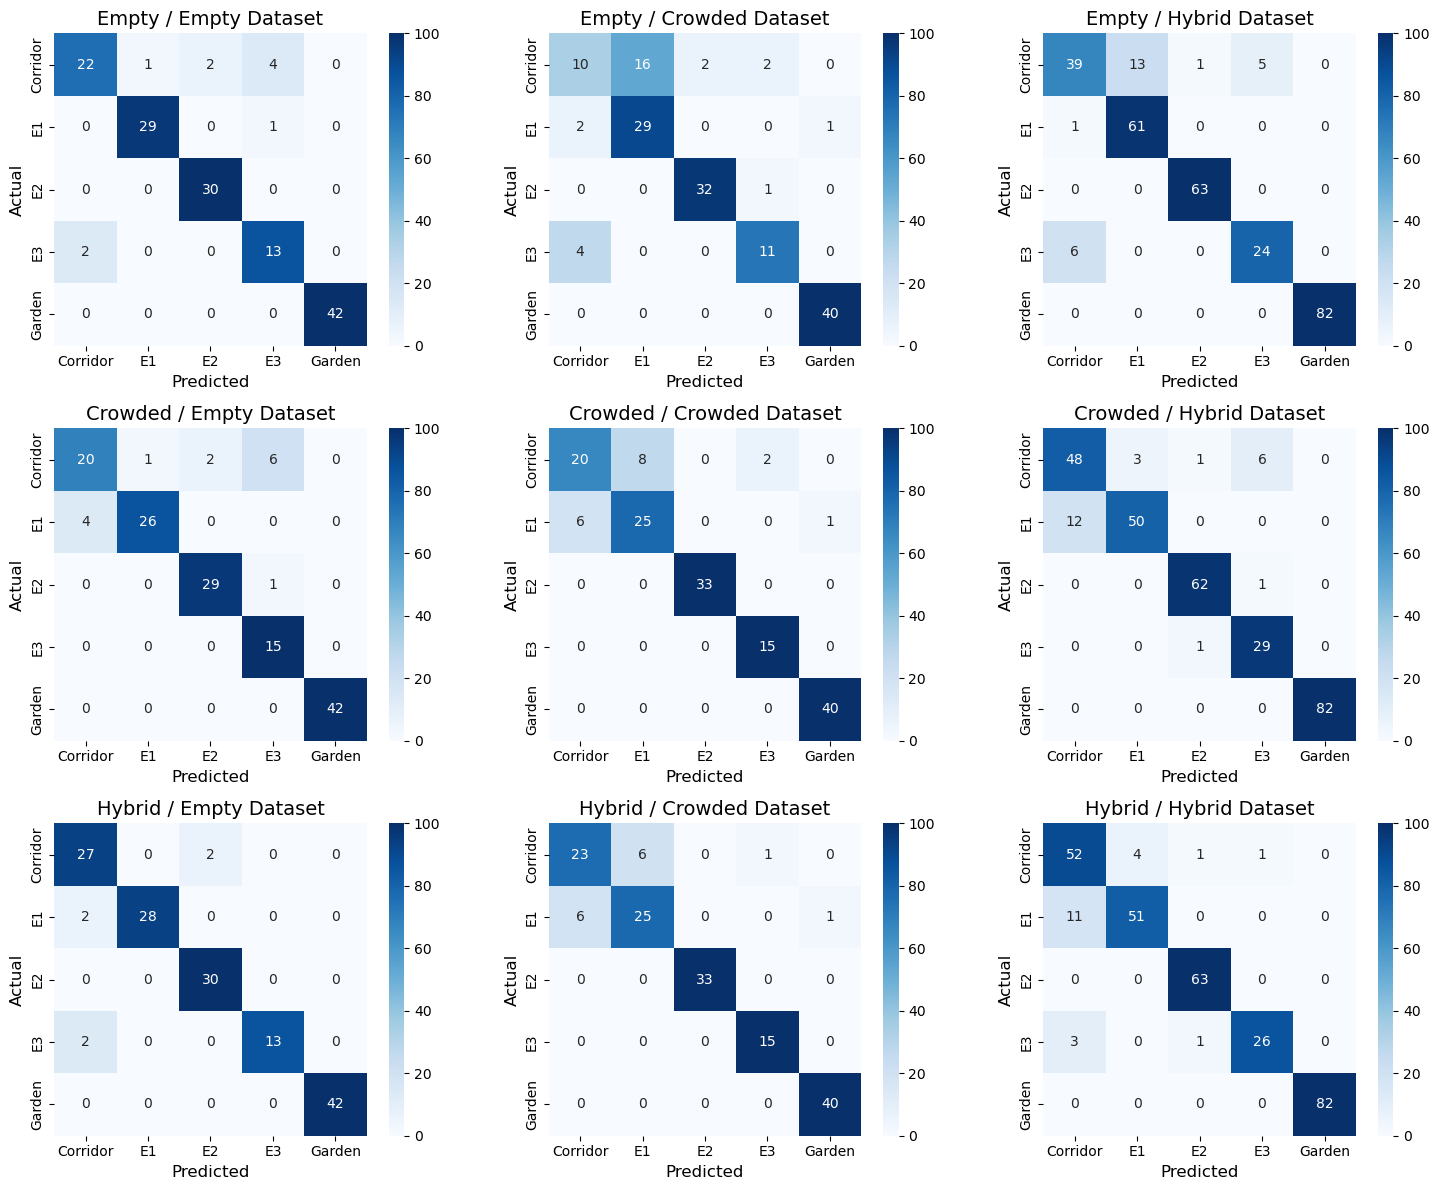
\includegraphics[scale=0.39]{img/MCGSCV.png}}
    \caption{Matrici di confusione ottenute dal modello KNN ottimizzato (GridSearchCV) su dataset \textit{Binarized}}
    \label{MCGtid}
\end{figure} 

Dall'analisi delle matrici di confusione riportate in \autoref{MCGtid} e dai dati in \autoref{tab:model_metrics}, emerge che il modello presenta in generale \textbf{prestazioni migliori quando il dataset di addestramento e quello di test coincidono}, ma con un'importante eccezione: \textbf{il caso \textit{Crowded--Crowded} risulta infatti quello con le prestazioni peggiori in assoluto}, con un'accuratezza inferiore rispetto anche a combinazioni in cui train e test avvengono su scenari differenti.\\
Il dataset \textbf{\textit{Hybrid} si conferma quello con la maggiore capacità di adattamento}, in quanto il modello è allenato su tutte le situazioni possibili, permettendo quindi una classificazione globalmente più accurata. \\

Considerati i buoni livelli di accuratezza raggiunti per tutte le configurazioni, si può dedurre inoltre che la \textbf{presenza di folla} all'interno delle aule \textbf{non sia un fattore particolarmente rilevante} ai fini della localizzazione, anche se sembra introdurre maggiore variabilità e rumore nei dati.\\

Gli \textbf{errori} più frequenti si verificano tra \textbf{``Corridor'' ed ``E1''}: sono due ambienti aventi la superficie in comune più estesa (\autoref{Pianta}). Probabilmente, a causa della posizione dei rispettivi router, i segnali Wi-Fi si sovrappongono creando confusione nella previsione e aumentando la probabilità di errori di classificazione.\\
\textbf{``Garden''} viene \textbf{classificato correttamente} nella maggior parte dei casi: anche in questo caso la motivazione deriva dalla sua posizione all'interno dello spazio considerato. Essendo separato distintamente dalle altre stanze considerate, il modello ha una maggiore facilità nel riconoscerlo.

\section{Conclusione}
In questo studio abbiamo analizzato l'efficacia del \textit{WiFi fingerprinting} per la localizzazione, valutando i vantaggi e le sfide di questo approccio. I risultati ottenuti \textbf{confermano la fattibilità del metodo}, pur evidenziando alcune limitazioni e possibili miglioramenti.

Il nostro studio ha dimostrato che l'uso di questa tecnica, anche con l'applicazione di un modello relativamente semplice come \textbf{KNN}, consente una localizzazione sufficientemente precisa: i risultati evidenziano che è \textbf{possibile individuare un utente all'interno del Dipartimento di Informatica utilizzando esclusivamente le onde radio emesse dai router AlmaWIFI}.

\subsection{Sviluppi futuri}
Il modello sviluppato potrebbe non essere sufficientemente robusto nel caso di \textit{modifiche alle stanze considerate}. Ad esempio, se venissero incluse le due aree in grigio di \autoref{Pianta} o, addirittura, se fosse necessario cambiare edificio, è possibile che il sistema implementato con questo approccio non fornisca più risultati soddisfacenti.\\

Una possibile espansione del lavoro potrebbe essere orientata verso una \textit{maggiore granularità nella localizzazione}. Invece di limitarsi a individuare la singola stanza, potrebbe essere interessante poter localizzare un'area più precisa all'interno della stanza stessa.\\

Per affrontare questo nuovo obiettivo, sarebbe necessario \textit{raccogliere un dataset più ampio o adottare metodologie alternative}, come ad esempio registrare la posizione esatta in cui vengono rilevati i segnali.\\

Questa espansione del dataset potrebbe anche rappresentare un'opportunità per esplorare e \textit{risolvere il problema utilizzando modelli più avanzati}, come SVM e Random Forest, che potrebbero contribuire a migliorare ulteriormente le prestazioni del sistema di localizzazione.


%%%%%%%%%%%%%%%%%%%%%%%%%%
\newpage
\bibliography{references}

\end{document}
